\chapter{Optimizing Photovoltaic Systems}\label{chapter:optimizing_pv_systems}

In this final chapter, \textbf{Optimizing Photovoltaic Systems}, we explore the
surrounding infrastructure around the solar array that enables it to operate at
its full potential. In particular, we take a look at the \acf{MPPT} \acf{HW}
used to control the solar array and propose a suite of MPPT algorithms that can
address nonidealities in the \ac{I-V} curve that were observed in
\autoref{sec:modeling_solar_arrays} such as global and local \acfp{MPP} and partial
shading effects. We present a comprehensive \ac{PV} system simulator that
incorporates the models discussed in \autoref{chapter:modeling_pvs} and the
high level design developed in \autoref{chapter:optimizing_pvs} to evaluate the
effects of these \ac{MPPT} algorithms in terms of stability, convergence speed,
total efficiency, and so forth. Finally, we implement a set of performant
algorithms in real \ac{HW} and validate that the optimizations and models
perform as expected.

\todo[inline,caption={}]{
    \begin{enumerate}
        \item Discuss process of energy conversion, losses at each step, build
        sankey diagram
        \item Introduce MPPT, MPPT algorithms
        \begin{itemize}
            \item General theory, objective for MPPTs
            \item Heuristics for solving constrained, multimodal surface
            optimization problems
            \item Briefly discuss prior art
            \begin{itemize}
                \item Esram et Chapman, Comparison of Photovoltaic Array Maximum
                Power Point Tracking Techniques
                \item Hill climbing algorithms
            \end{itemize}
            \item Focus on interesting variations and novel techniques
            \begin{itemize}
                \item Hill climbing algorithms - sublocal stride algorithms
                (Fixed, Optimal, Adaptive, Bisection stride)
                \item Divide and conquer algorithms
                \begin{itemize}
                    \item Ternary search
                    \item Golden section search
                    \item Bisection method search
                \end{itemize}
                \item Metaheuristic optimization algorithms
                \begin{itemize}
                    \item Simulated annealing
                    \item Particle swarm optimization
                \end{itemize}
                \item Other algorithms
                \begin{itemize}
                    \item Voltage sweep
                    \item Fuzzy logic controllers
                    \item Newton-Raphson method
                    \item Trapezium method
                    \item Artificial neural networks
                \end{itemize}
            \end{itemize}
            \item Issues with `local' and `global' algorithms
            \item Propose a multi-hierarchical MPPT algorithm framework
            \begin{itemize}
                \item Optimizing goals for each part of the hierarchy
                \item Proposed clusterings of algorithms
            \end{itemize}
        \end{itemize}
    \end{enumerate}
}

\todo[inline,caption={}]{
    \begin{enumerate}
        \setcounter{enumi}{3}
        \item Present a model for DC-DC converter and how it works in relation
        to an MPPT (bridge HW to SW)
        \item Present system simulator
        \begin{itemize}
            \item Environmental modeling
            \item Array modeling
            \item MPPT algorithm modeling
        \end{itemize}
        \item Simulator results
        \begin{itemize}
            \item Impulse response (look at steady state behavior)
            \item Step response (look at convergence speed, steady state behavior)
            \item Simulated environmental profile response
            \item Efficiency analysis and metrics, figure of merit
        \end{itemize}
        \item Introduce MPPT HW and how MPPT algorithms were implemented in HW
        (likely move to Appendix)
        \item Real world testing results
    \end{enumerate}
}




\begin{figure}[h]
    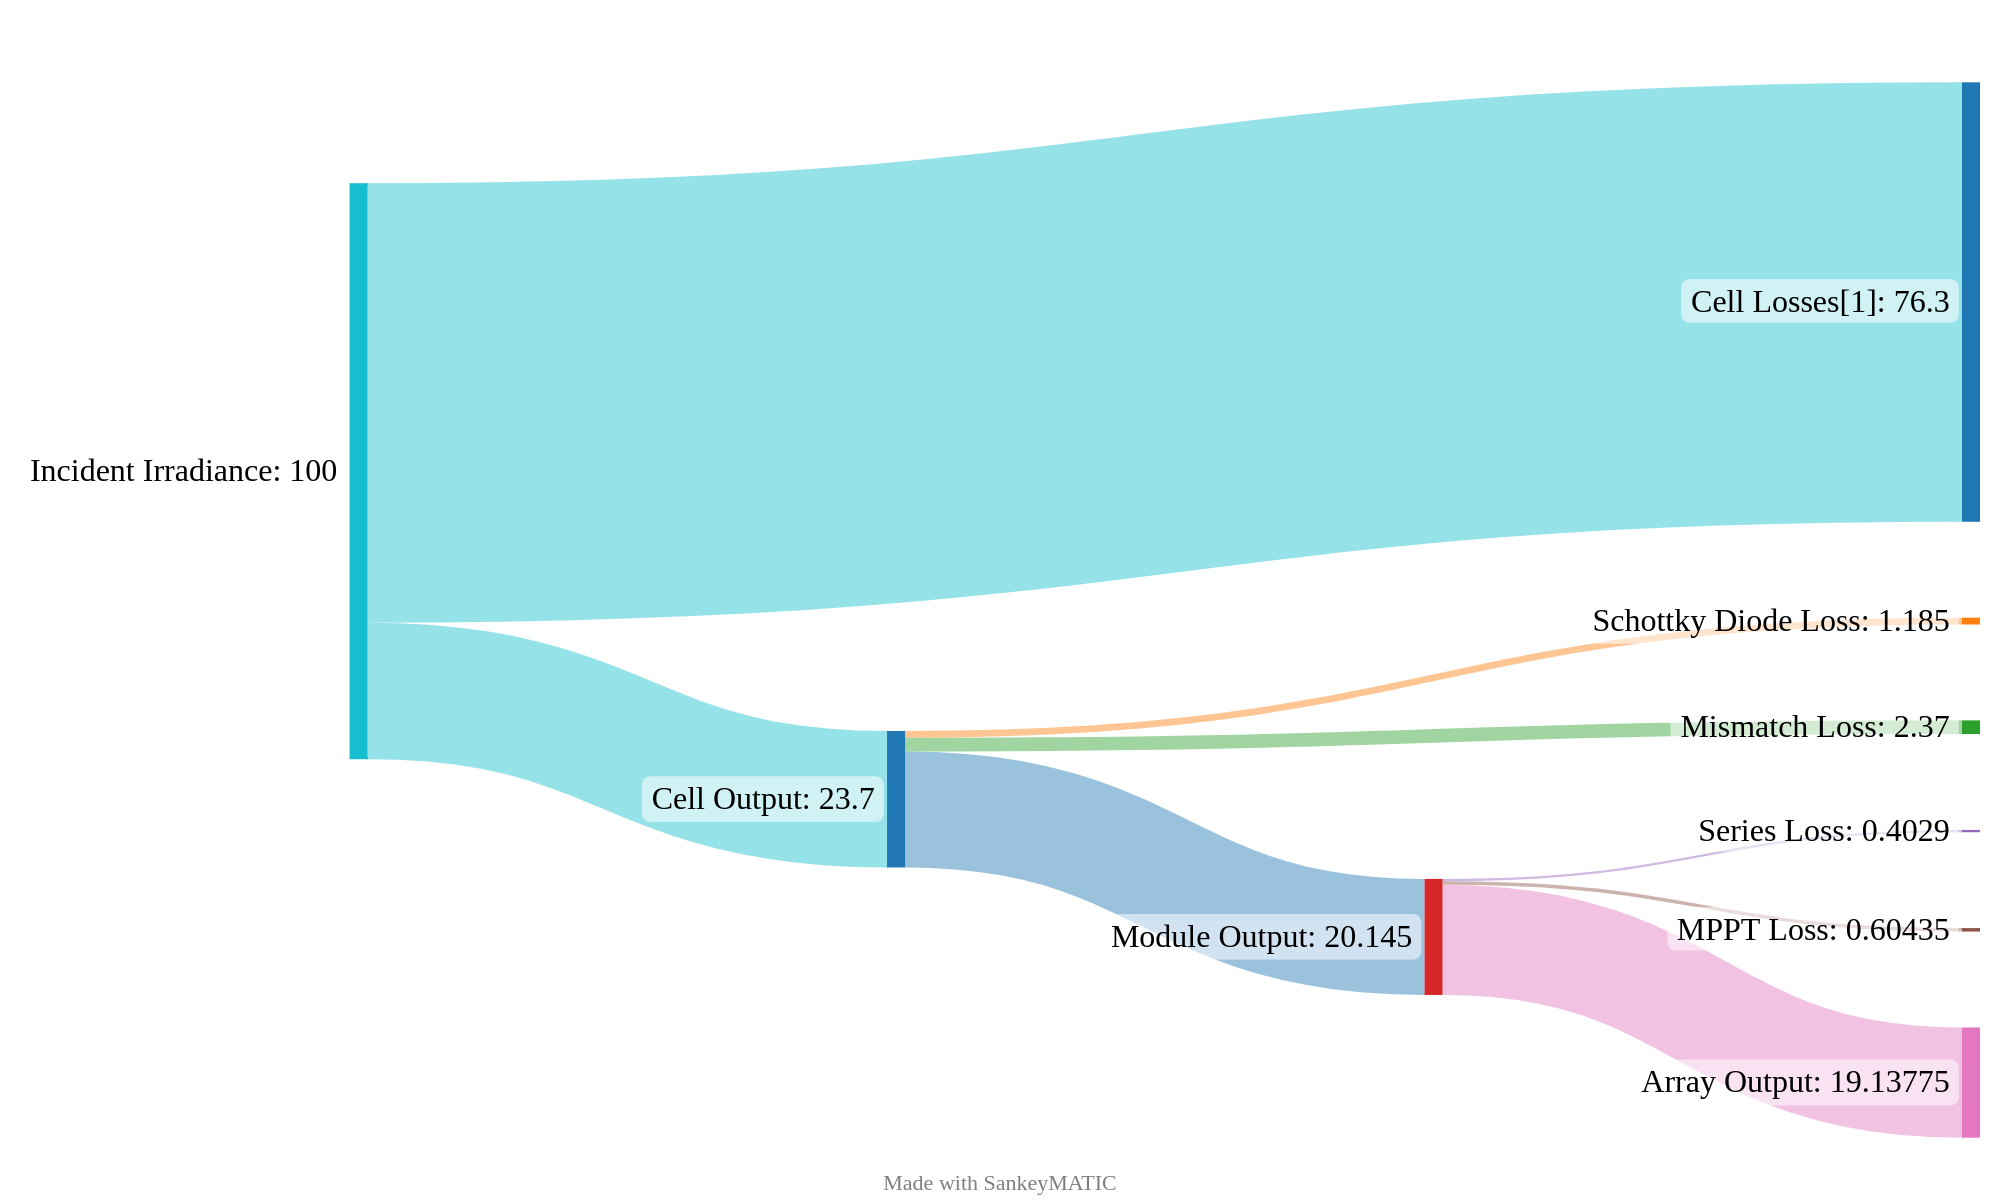
\includegraphics[width=\textwidth]{photovoltaic_system_sankey.png}
    \caption{Sankey Diagram for Photovoltaic System}
    \label{fig:photovoltaic_system_sankey}
\end{figure}

\todo[inline]{Reset sankey with real data}


\section{Conclusion}\label{sec:optimizing_pv_systems_conclusion}

%TODO: conclusion for Chapter 3
\todo[inline]{Insert conclusion on chapter topics and results.}

